%% SMART-ANN --- IEEE conference paper (IEEEtran, conference mode).
%%
%% Build:  pdflatex main && bibtex main && pdflatex main && pdflatex main
%% Figures: run `python scripts/make_paper_figures.py` first; it writes
%% results/paper/*.pdf from the recorded results. Every number in this paper
%% is traceable to a file under results/ --- see Section IV.
\documentclass[conference]{IEEEtran}
\IEEEoverridecommandlockouts

\usepackage{cite}
\usepackage{amsmath,amssymb}
\usepackage{graphicx}
\usepackage{booktabs}
\usepackage{url}
\usepackage[hidelinks]{hyperref}
\usepackage{balance}

\graphicspath{{../results/paper/}}

\def\BibTeX{{\rm B\kern-.05em{\sc i\kern-.025em b}\kern-.08em
    T\kern-.1667em\lower.7ex\hbox{E}\kern-.125emX}}

\begin{document}

\title{Spend Effort Where It Buys Something: Query-Difficulty-Conditioned
Retrieval Control for On-Device RAG}

% One shared block rather than three side by side. All three authors have the
% same affiliation, so repeating it three times bought nothing and pushed the
% block onto a second row, which cost roughly 1.7 column-inches -- enough to
% spill the last two references onto a page of their own.
\author{\IEEEauthorblockN{Anshuman Kumar, Govind Mukund Agarwal, and Shivam Kumar}
\IEEEauthorblockA{\textit{School of Computer Science and Engineering},
\textit{Vellore Institute of Technology}, Vellore, India \\
anshuman.kumar@vitstudent.ac.in,
govind.mukund2023@vitstudent.ac.in,
shivam.kumar2023c@vitstudent.ac.in}
}

\maketitle

\begin{abstract}
On-device retrieval-augmented generation (RAG) runs on a fixed battery with no
fan, so every millisecond of retrieval is heat and charge that cannot be
recovered. Existing mobile RAG indexes fix their search parameters at build
time and therefore spend identical effort on every query. We observe that a
two-phase disk-resident IVF index already computes, for free, a signal that
predicts how much effort a query needs: the distance gap between the nearest
and second-nearest centroid, available before a single cluster is opened. On a
46{,}369-passage SQuAD index we measure that this signal separates recall@10 at
the cheapest effort level from $0.278$ to $0.978$ across difficulty
quintiles---a $3.5\times$ spread---and that one step of additional effort is
worth $+0.403$ recall to the hardest fifth of queries and $+0.009$ to the
easiest, a $45\times$ difference in marginal value. We fit an effort allocation
against a profile table of latencies measured on a physical handset and
validate it on 500 held-out queries: at near-equal device cost it improves
recall@10 on three of five budgets, by up to $+0.0162$ against a resolution
floor of $0.0002$. We further report a negative result that we believe is
useful to anyone building thermally-aware mobile systems: across six recorded
handset runs the Android skin sensor never reached the $42\,^{\circ}$C
threshold at which our thermal policy derates, while the hottest internal
thermal zone exceeded it in all six, peaking at $78.8\,^{\circ}$C against a
skin peak of $37.5\,^{\circ}$C. A thermal shield reading the conventional
sensor never trips. All measurements, including the ones that failed, are
reproducible from the released artifact.
\end{abstract}

\begin{IEEEkeywords}
on-device retrieval, retrieval-augmented generation, approximate nearest
neighbor search, adaptive control, energy efficiency, mobile systems
\end{IEEEkeywords}

\section{Introduction}

Retrieval-augmented generation grounds a language model's output in retrieved
documents~\cite{lewis2020rag,gao2023ragsurvey}. Moving that pipeline onto a
phone is attractive for privacy and for offline operation, but it changes the
cost model completely. A datacenter retrieval system trades latency against
accuracy; a phone trades latency, accuracy, \emph{heat} and \emph{charge},
against a battery that does not refill during the session and a chassis with no
active cooling. The energy cost of language technology has been argued at the
scale of training runs~\cite{strubell2019energy,schwartz2020greenai}; on a
handset the same argument applies per query, to a budget the user can watch
draining.

MobileRAG~\cite{park2025mobilerag} is the current reference design for this
setting. Its EcoVector index keeps an HNSW graph over IVF centroids resident in
RAM and stores each cluster's vectors on disk, so that answering a query touches
only the clusters it chooses to open. This is the right shape for a phone. But
its search parameters---chiefly \texttt{nprobe}, the number of clusters
opened---are fixed at build time. Every query therefore receives identical
effort, regardless of how hard that query is and regardless of what state the
device is in.

Uniform allocation is a strange default given the shape of the underlying
curve. Figure~\ref{fig:effort} plots our handset-measured cost against recall:
going from one cluster to four costs $38$~ms and buys $0.20$ recall; going from
sixteen to thirty-two costs $164$~ms and buys $0.03$. The curve is steep at one
end and flat at the other, which is precisely the condition under which
\emph{who gets the effort} matters more than \emph{how much effort there is in
total}.

This paper makes that reallocation concrete. Our central observation is that
the information needed to do it is already being computed and thrown away. A
two-phase index must first search its centroid structure to decide which
clusters to open; that search produces, at no additional cost, a measure of how
decisively one cluster won. We show that this measure predicts query difficulty
well enough to beat uniform allocation at equal cost.

\subsection*{Contributions}

\begin{enumerate}
\item \textbf{Query-difficulty-conditioned effort allocation from a free
signal} (Section~\ref{sec:c6}). We identify the centroid distance gap, already
computed by the probe phase of a two-phase IVF index, as a difficulty predictor
available \emph{before} any expensive work. We fit an allocation against
handset-measured costs and validate it on held-out queries. To our knowledge
this is the first use of a probe-time difficulty signal to allocate retrieval
effort under a \emph{device-measured} cost budget on a mobile index; the
closest prior work adapts the RAG strategy above the index rather than the
search effort inside it, and pays for a trained classifier to do it
(Section~\ref{sec:rel-adaptive-rag}).

\item \textbf{A measured negative result on thermal sensor selection}
(Section~\ref{sec:sensors}). Across six recorded runs on a physical handset,
the sensor that Android exposes as ``skin temperature'' and the hottest
internal thermal zone diverge by $20.1$ to $41.3\,^{\circ}$C at peak. A policy
whose thresholds are calibrated on skin temperature---as ours was, and as we
argue is the natural choice---never trips on runs that recorded a
$78.8\,^{\circ}$C component. We report this as a failed contribution rather
than removing it.

\item \textbf{Per-query energy measured rather than extrapolated}
(Section~\ref{sec:energy}). On an unplugged handset over $9{,}670$ queries we
measure $130.99$~mJ per query all-in and a marginal cost of $3.21$~mJ per
cluster opened, with median power rising $97.6\%$ from the quietest to the
busiest quintile of retrieval work.

\item \textbf{A measurement discipline that makes absence visible}
(Section~\ref{sec:method}). Every number we report is traceable to a file
written by a recorded run; quantities the platform could not measure propagate
as \texttt{NaN} rather than defaulting; and one derived quantity is
\emph{refused} outright because its inputs were contaminated. We describe this
because it changed our results twice.
\end{enumerate}

\begin{figure*}[t]
\centering
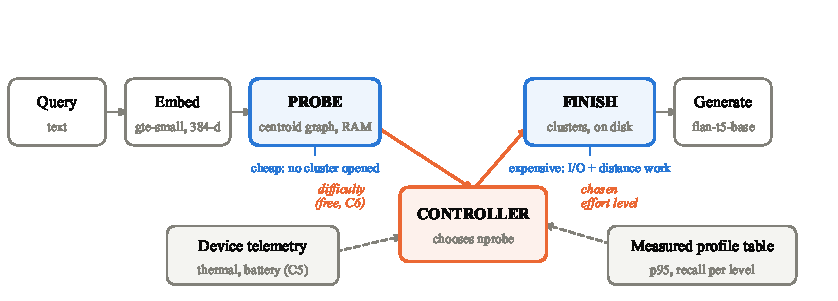
\includegraphics[width=\textwidth]{fig1_architecture.pdf}
\caption{The pipeline, and where each control signal enters. The probe phase
searches only the centroid graph and opens no clusters; the finish phase pays
the I/O and distance cost. The controller sits between them, which is what
makes per-query allocation possible at all: the difficulty signal
(Section~\ref{sec:c6}) is a by-product of the cheap phase and is available
before the expensive one commits. Device telemetry (Section~\ref{sec:sensors})
enters the same decision point.}
\label{fig:arch}
\end{figure*}

\section{Background and Related Work}

\subsection{Two-phase disk-resident ANN indexes}

Inverted-file (IVF) indexes partition a corpus into $N_c$ clusters and search
only the \texttt{nprobe} nearest ones~\cite{johnson2021faiss,douze2024faiss}.
Graph indexes such as HNSW~\cite{malkov2020hnsw} give better recall per distance
computation but require the whole graph resident. Disk-resident designs such as
DiskANN~\cite{subramanya2019diskann}, SPANN~\cite{chen2021spann} and
EcoVector~\cite{park2025mobilerag} combine the two: a small structure in memory
decides where to look, and the bulk stays on disk. Our index follows EcoVector:
an HNSW graph over $215$ centroids in RAM, each cluster's vectors memory-mapped
from its own file. Recall against latency on such indexes is conventionally
reported as a curve rather than a point~\cite{aumuller2020annbench}, and
Section~\ref{sec:c6} argues that the curve's asymmetry is itself the
opportunity.

The consequence that matters here is structural. Because the design is
two-phase, there is a decision point between a cheap phase and an expensive
one. Single-phase designs have no such point, which is why the mechanism we
describe is specific to this family of indexes rather than general to ANN
search.

EdgeRAG~\cite{seemakhupt2024edgerag} is the closest system to ours in
intent: it keeps first-level centroids resident and generates the second level
online, for RAG on edge hardware. Its evaluation platform is a Jetson Orin---an
embedded GPU board with a heatsink and wall power. That difference is the reason
thermal state and charge enter our control law at all, and the reason our costs
come from a phone rather than from a board.

\subsection{Adaptive ANN search}

Adaptivity in ANN search is not new. Li et
al.~\cite{li2020earlytermination} learn to terminate graph search early on a
per-query basis, predicting from intermediate search state when further
exploration will not improve the result. Our approach differs in two ways that
matter for the mobile setting. First, their signal is observed \emph{during}
search, so the decision is a stopping rule; ours is observed \emph{before}
search from the probe's own output, so the decision is a budgeting rule and the
work is never started. Second, and more importantly for a phone, their
objective is latency on a server; ours is allocation against a table of
latencies measured on the target handset, so the optimiser trades recall
against milliseconds that were actually observed on the device that will run
the query.

DARTH~\cite{chatzakis2025darth} makes the case for adaptivity more sharply
still, and from the same premise we start from: a single fixed parameter
setting gives good recall on some queries and poor recall on hard ones, so a
declarative recall target is better served by terminating per query, with
reported speedups up to $41.8\times$ on IVF indexes. The distinction from our
work is the one we draw above. DARTH decides when to stop once search is under
way; we decide what to spend before it starts. The two are compatible---a
budget chosen from difficulty could be terminated early by a recall target---and
we see that composition as the natural next step rather than a competing design.

Anisotropic quantisation~\cite{guo2020scann} and related work improve the
accuracy-per-byte of the index itself. That is orthogonal: a better index
changes the profile table our controller reads, and the controller keeps
working.

\subsection{Adaptive retrieval in RAG pipelines}
\label{sec:rel-adaptive-rag}

A parallel line of work adapts the \emph{RAG strategy} rather than the search
inside it. Adaptive-RAG~\cite{jeong2024adaptiverag} is the closest prior work
to ours in spirit: it routes each question to no retrieval, single-step
retrieval or iterative retrieval according to a predicted complexity class.
Self-RAG~\cite{asai2024selfrag} has the model itself decide when to retrieve
and critique what it retrieved; FLARE~\cite{jiang2023flare} triggers retrieval
mid-generation when the model's own confidence drops; and Mallen et
al.~\cite{mallen2023whennot} show that retrieval helps unevenly across
questions, which is the empirical premise all of these rest on.

Our work differs from this line on three axes, and we think the first is the
one that matters.

\emph{The lever.} These systems choose how many \emph{LLM and retrieval calls}
to make. We choose how much \emph{ANN search effort} to spend inside a single
retrieval---how many clusters to open. The two are orthogonal: an
Adaptive-RAG router could sit above our controller, and each query it routed to
retrieval would still face the question of how hard to search.

\emph{The cost of the signal.} Adaptive-RAG's complexity classifier is a trained
model with its own training data and its own inference cost on the query path.
Our signal is a by-product of work the index performs regardless, costs nothing
additional, and requires no training---which is what makes it viable on a device
where the classifier's own forward pass would be a measurable fraction of the
budget it is trying to manage.

\emph{The cost axis.} Their objective is answer quality against LLM calls. Ours
is recall against milliseconds and joules measured on the handset that will run
the query.

\subsection{Resource-aware mobile inference}

Thermal and energy management for on-device inference is an active area, and
the standard lever is DVFS or model switching. Benchmarking infrastructure for
this setting is maturing: MELT~\cite{laskaridis2024melt} traces language-model
workloads on real handsets at fine granularity, covering performance, energy
and thermal behaviour together, and the AI Benchmark
series~\cite{ignatov2019aibench} established the practice of reporting
smartphone inference across devices rather than on one. Our measurement
apparatus (Section~\ref{sec:method}) is in that tradition, applied to retrieval
rather than to generation.

We are not aware of prior work that treats \emph{retrieval effort} as the
controlled variable on a phone, with the control law reading device telemetry.
Section~\ref{sec:sensors} reports what happened when we tried, including why it
did not work.

\section{System Design}

\subsection{Index and pipeline}

Our corpus is the SQuAD~\cite{rajpurkar2016squad} development passages,
sentence-windowed into $46{,}369$ chunks and embedded to 384 dimensions with a
\texttt{gte-small} encoder~\cite{li2023gte}, L2-normalised, searched under
inner product---the dense single-vector retrieval setting established by
DPR~\cite{karpukhin2020dpr}. The index is built with $N_c = 215$ clusters.
Answer generation uses \texttt{flan-t5-base}~\cite{chung2024flan} with greedy
decoding.

A query proceeds as in Figure~\ref{fig:arch}. It is embedded; the
\emph{probe} phase searches the resident centroid graph and returns the
clusters ranked by distance; the controller chooses \texttt{nprobe}; the
\emph{finish} phase opens exactly that many cluster files and merges their
results by true distance; the retrieved passages are assembled into a prompt
and generated from.

\subsection{The profile table}

The controller does not predict cost from a model. It chooses from a table of
\emph{measured} costs, one row per effort level, recorded on the target handset
(Table~\ref{tab:profile}, plotted in Figure~\ref{fig:effort}). Each row is the
p95 latency and recall@10 over $3{,}829$ queries executed on the device.

\begin{table}[t]
\caption{Profile table: effort levels as measured on the handset (vivo I2304),
$3{,}829$ queries per level. The controller selects a row; it does not
interpolate between them.}
\label{tab:profile}
\centering
\begin{tabular}{rrrr}
\toprule
\texttt{nprobe} & p50 (ms) & p95 (ms) & recall@10 \\
\midrule
1  & 5.59   & 13.82  & 0.6405 \\
4  & 20.50  & 52.26  & 0.8417 \\
8  & 40.46  & 101.46 & 0.9065 \\
16 & 82.61  & 189.82 & 0.9507 \\
32 & 169.21 & 354.10 & 0.9788 \\
\bottomrule
\end{tabular}
\end{table}

\begin{figure}[t]
\centering
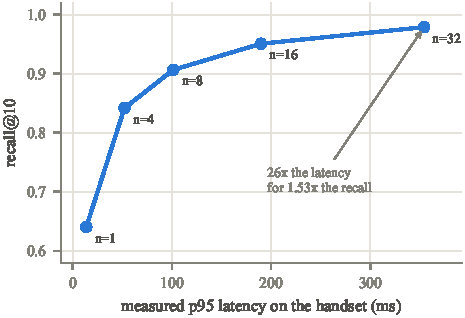
\includegraphics[width=\columnwidth]{fig2_effort_return.pdf}
\caption{The curve the controller chooses from, measured on the handset. The
first $38$~ms of additional latency buys $0.20$ recall; the last $164$~ms buys
$0.03$. A curve this asymmetric is why allocation matters.}
\label{fig:effort}
\end{figure}

We use a measured table rather than the analytic cost model we also fitted,
because that model fails where it matters. Fitted on quiet phases of three runs
($21{,}388$ samples) it reaches $14.75\%$ MAPE, inside our declared $15\%$
target; held out on contended phases it degrades to $35.87\%$. A predictor that
is most wrong when the CPU is busiest would choose the wrong level exactly when
choosing right matters most.

\subsection{Policies}

All policies select a row of the profile table. \textsc{Static} fixes a level.
\textsc{Budget} selects the highest-recall row whose measured p95 fits a
declared latency target (with $0.9$ headroom). \textsc{Aimd} adjusts
multiplicatively from observed latency. \textsc{Device} composes over
\textsc{Budget} and may only \emph{lower} the level it chose, on thermal or
battery grounds. \textsc{QueryAdaptive} (Section~\ref{sec:c6}) likewise
composes over \textsc{Budget} and may only lower.

That composition rule is deliberate. A policy able to raise effort above the
budget---because it judged a query hard, or because it wanted to finish before
the device got hotter---could miss the declared latency target in the service
of some other goal. No such trade was declared, so no policy is permitted to
make it.

\section{Measurement Methodology}
\label{sec:method}

This section describes how we decided what we were allowed to claim. We include
it because the discipline changed our results twice, and because a reader
judging the negative result in Section~\ref{sec:sensors} needs to know it was
not simply a run we chose not to debug.

\subsection{Absence is represented, not defaulted}

Every telemetry field the platform cannot supply is \texttt{NaN}, never zero.
Every policy that reads a device signal checks for finiteness and declines to
act on an absent one. The distinction is load-bearing: a laptop with no
thermometer and a phone at $27\,^{\circ}$C both produce an empty list of
reasons from the thermal policy, and reporting those identically would present
the absence of a measurement as a measurement of good health.

\subsection{Derived quantities may be refused}

We fitted a first-order lumped thermal model,
$\mathrm{d}T/\mathrm{d}t = a\,w + b\,(T - T_{\mathrm{ref}}) + c$, obtaining a
time constant $\tau = 67.9$~s ($R^2 = 0.30$). We use $\tau$, because a
controller acting faster than the thermal observation delay is acting on noise.
We \emph{refuse} to use the same fit to decompose a temperature rise into
contributions, because the trace it was fitted on was recorded with the handset
on AC power: charger heat is absorbed into the constant term $c$, so $c$ is not
the device's idle thermal state. An early version of this decomposition
attributed $+216\,^{\circ}$C to retrieval on a run whose thermometer moved
$5.6\,^{\circ}$C. Rather than drop the offending term, the entire decomposition
is refused and reported as refused.

\subsection{Held-out validation for anything fitted}

The allocation in Section~\ref{sec:c6} is fitted on one half of the query set
and scored on the other, with the split fixed by seed. Difficulty buckets fitted
and then evaluated on the same queries would measure memorisation, and would
produce a real-looking number.

\subsection{A resolution floor is stated}

With $500$ held-out queries at $k=10$, one query gaining one neighbour moves
mean recall by exactly $1/(500 \times 10) = 0.0002$. We report this floor beside
every difference so that a reader can see whether an effect is an effect or four
queries.

\subsection{What is measured where}

Retrieval was executed on a physical handset (vivo I2304): the profile table,
the policy comparison of Section~\ref{sec:c5}, and the energy measurements are
all on-device, totalling $39{,}438$ recorded queries in the run used for
Section~\ref{sec:c5} alone. Generation was \emph{not} run on the handset;
generation timings in our pipeline are host numbers and are labelled as such
throughout. Recall is a property of the index and the query rather than of the
machine---the same query at the same \texttt{nprobe} returns the same
neighbours anywhere---so recall measured on the host transfers unchanged, and
we rely on that in Section~\ref{sec:c6} while taking every cost from the
handset table.

\section{Effort Allocation by Query Difficulty}
\label{sec:c6}

\subsection{The signal}

When the probe phase searches the centroid graph it obtains the distances to
the nearest centroids. We define the difficulty signal as the gap between the
two nearest:
\begin{equation}
g = d_2 - d_1 ,
\end{equation}
a difference rather than the ratio $d_2/d_1$ that would be the obvious choice.
The ratio divides by a distance that can be zero or negative: for duplicate
vectors under inner product on L2-normalised float32 rows, $1 - \langle q,c
\rangle$ can land marginally below zero. The difference carries the same
information and is always defined.

A large $g$ means one cluster decisively won and the true neighbours are
probably inside it. A small $g$ means the query sits between clusters and its
neighbours are scattered across them, so a search that opens few clusters will
miss them.

Critically, $g$ costs nothing. It is a by-product of work the index must do
regardless, and it is available before any cluster file is touched.

\subsection{The signal separates, and by a large margin}

Figure~\ref{fig:difficulty}(a) shows recall@10 against effort for queries
bucketed into quintiles of measured $g$. At \texttt{nprobe}~$=1$ the hardest
quintile recovers $0.278$ of the true neighbours and the easiest recovers
$0.978$. That is a $3.5\times$ spread, produced by a quantity the index
computes for free.

Figure~\ref{fig:difficulty}(b) is the operational form of the same fact: what
one step of additional effort is worth. Moving from \texttt{nprobe}~$1$ to $4$
buys the hardest quintile $+0.403$ recall and the easiest $+0.009$---a
$45\times$ difference in the marginal value of a cluster. Under uniform
allocation both quintiles receive the same increment.

\begin{figure*}[t]
\centering
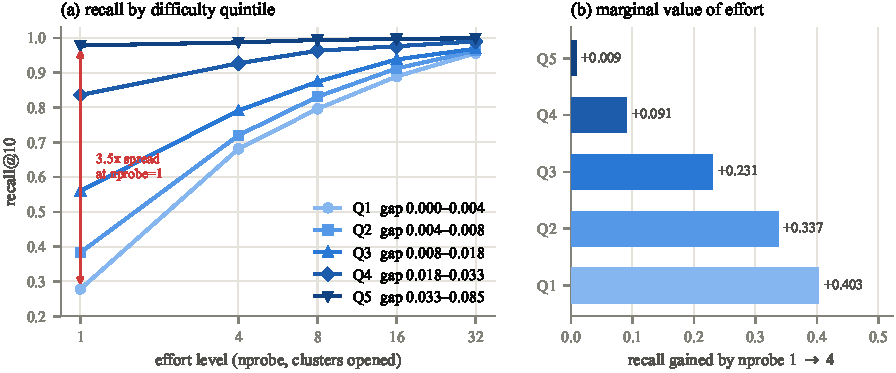
\includegraphics[width=\textwidth]{fig3_difficulty.pdf}
\caption{The observation the method rests on, on $1{,}000$ SQuAD queries. (a)
Recall@10 against effort, by quintile of the probe-time difficulty signal; the
quintiles are ordered, so they are drawn as one hue stepped light to dark. At
the cheapest level the quintiles are separated by a factor of $3.5$. (b) The
marginal value of one step of effort differs by $45\times$ between the hardest
and easiest quintile. Uniform allocation gives both the same step.}
\label{fig:difficulty}
\end{figure*}

\subsection{Fitting an allocation}

Let $B$ be a set of difficulty buckets with population weights $w_b$, $L$ the
set of effort levels, $r_{b\ell}$ the measured mean recall of bucket $b$ at
level $\ell$, and $c_\ell$ the handset-measured p95 cost of level $\ell$. For a
cost budget $C$ we solve~(\ref{eq:alloc}):
\begin{equation}
\max_{\ell : B \to L} \ \sum_{b \in B} w_b\, r_{b \ell(b)}
\quad\text{s.t.}\quad \sum_{b \in B} w_b\, c_{\ell(b)} \le C .
\label{eq:alloc}
\end{equation}

Three properties of this formulation are deliberate. The bucket edges are
quantiles of the \emph{measured} $g$ distribution rather than chosen
thresholds. The objective and the constraint are both populated entirely by
measurements---$r_{b\ell}$ from a recall sweep, $c_\ell$ from the handset. And
with five buckets and five levels the search space is $5^5 = 3125$
assignments, so we enumerate it exhaustively: the optimum is exact and there is
no solver tolerance to justify.

We instantiate $C$ at each level's own cost, so that every comparison replaces
a uniform policy with an allocation of the same nominal budget.

\subsection{Held-out result}

Buckets and allocation are fitted on $500$ queries and scored on the $500$ never
used for fitting (seed $0$). Table~\ref{tab:c6} and Figure~\ref{fig:c6} report
the outcome.

\begin{table}[t]
\caption{Effort allocation against uniform effort, on $500$ held-out queries.
Costs are handset-measured. The resolution floor is $0.0002$ recall per
query-neighbour.}
\label{tab:c6}
\centering
\begin{tabular}{lrrrrr}
\toprule
Budget & \multicolumn{2}{c}{recall@10} & $\Delta$ & \multicolumn{2}{c}{cost (ms)} \\
\cmidrule(lr){2-3}\cmidrule(lr){5-6}
 & uniform & allocated & & uniform & allocated \\
\midrule
\texttt{n}=1  & 0.6022 & 0.6022 & $+0.0000$ & 13.8  & 13.8 \\
\texttt{n}=4  & 0.8212 & \textbf{0.8304} & $+0.0092$ & 52.3  & 49.9 \\
\texttt{n}=8  & 0.8952 & \textbf{0.9114} & $+0.0162$ & 101.5 & 104.3 \\
\texttt{n}=16 & 0.9472 & \textbf{0.9562} & $+0.0090$ & 189.8 & 196.3 \\
\texttt{n}=32 & 0.9764 & 0.9758 & $-0.0006$ & 354.1 & 322.9 \\
\bottomrule
\end{tabular}
\end{table}

\begin{figure*}[t]
\centering
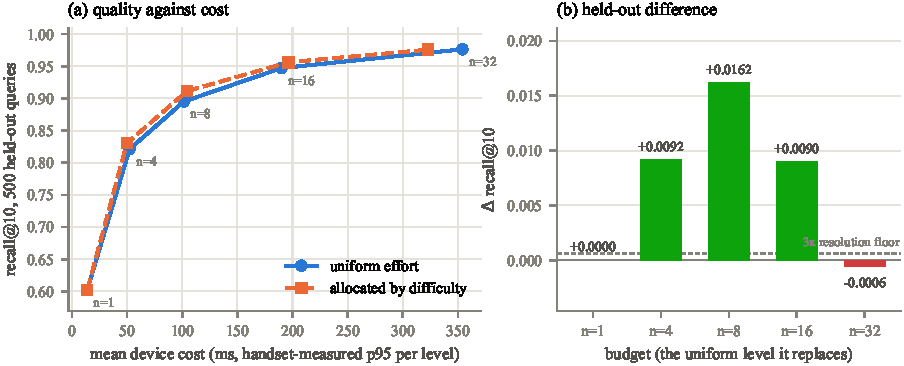
\includegraphics[width=\textwidth]{fig4_c6.pdf}
\caption{Allocation against uniform effort on $500$ held-out queries. (a) The
allocated curve sits above the uniform curve over the useful middle of the
range. (b) Per-budget difference, with the $3\times$ resolution floor marked.
Three budgets improve by margins well clear of it; the cheapest cannot improve
because every bucket is already at the floor level, and the most expensive
cannot because every bucket is near ceiling.}
\label{fig:c6}
\end{figure*}

Three of five budgets improve, by margins of $45$ to $81$ times the resolution
floor. The two that do not are explained by the allocation itself: at
\texttt{nprobe}~$=1$ the fitted assignment is $[1,1,1,1,1]$---there is no
cheaper level to move effort from---and at \texttt{nprobe}~$=32$ four of five
buckets are already above $0.95$ recall, so there is nothing left to buy.

\subsection{An honest statement of the cost axis}

The allocation is constrained to the budget on the fit half. The held-out half's
difficulty mix is not identical, so realised cost drifts in both directions: the
allocation spent $4.6\%$ and $8.8\%$ \emph{less} than the uniform arm at two
budgets, and $2.8\%$ and $3.4\%$ more at the two others. The comparison is
therefore at \emph{near}-equal cost, not exactly equal cost, and we state it
that way rather than reporting only the budgets where the drift favours us.

The budget with the largest recall gain is one where the allocation overspent:
$+1.8\%$ recall for $+2.8\%$ time. A reader entitled to be suspicious of that
should compare the alternative way of buying recall at this operating point.
Climbing the uniform curve from \texttt{nprobe}~$8$ to $16$ costs $+87\%$
latency for $+5.8\%$ recall---$0.067$ percentage points of recall per point of
latency, against the allocation's $0.66$. Per millisecond the allocation is
roughly an order of magnitude the better trade. It is a favourable exchange
rate, not a free lunch, and we make no stronger claim.

\section{Evaluation of the Control Layer}

\subsection{Budgeted control against static configuration}
\label{sec:policies}

Table~\ref{tab:policies} and Figure~\ref{fig:policies} compare three policies
against one latency budget, on one interleaved query stream. The budget
($14.01$~ms) was fixed from the profile table \emph{before} any policy ran, so
no policy is judged against a target derived from itself.

\begin{table}[t]
\caption{Three policies, one declared $14.01$~ms budget, interleaved on the same
query stream. Overhead is the controller's own decision cost as a fraction of
the query it governs.}
\label{tab:policies}
\centering
\begin{tabular}{lrrrr}
\toprule
Policy & queries & over budget & recall@10 & overhead p95 \\
\midrule
\textsc{Static} & 7{,}228  & 5.98\% & 0.8480 & 0.006\% \\
\textsc{Aimd}   & 8{,}790  & 4.31\% & 0.8103 & 0.131\% \\
\textsc{Budget} & 10{,}681 & \textbf{0.17\%} & 0.7797 & 0.167\% \\
\bottomrule
\end{tabular}
\end{table}

\begin{figure*}[t]
\centering
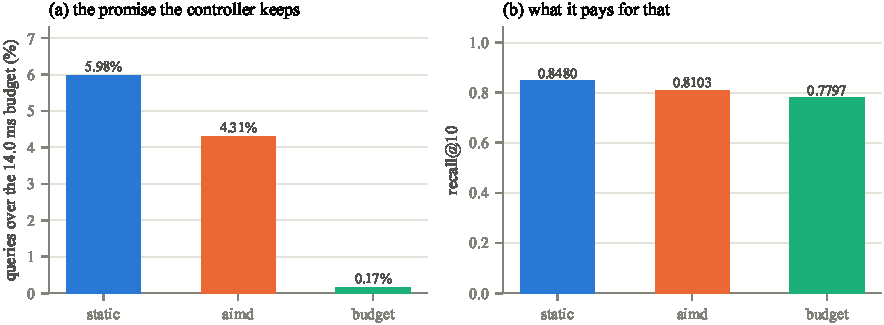
\includegraphics[width=\textwidth]{fig6_policies.pdf}
\caption{(a) The budgeted controller misses its latency target on $0.17\%$ of
queries against the static configuration's $5.98\%$, a $35\times$ reduction.
(b) It pays $0.068$ recall for that. Both panels are the same $26{,}699$
queries.}
\label{fig:policies}
\end{figure*}

The budgeted controller reduces deadline misses by $35\times$ and pays $0.068$
recall for it. We report both numbers because the trade is the result; a paper
that reported only the violation reduction would be describing half of what
happened. The controller's own decision costs at most $0.167\%$ of the query it
governs, so it is not consuming what it saves.

\textsc{Aimd} is included because it failed instructively. It reacts to
observed latency, and on a device whose thermal time constant is $67.9$~s
(Section~\ref{sec:method}) a controller reacting per query acts on noise. It
lands between the other two on both axes and is dominated by neither.

\subsection{Context reduction is a measured cost, not a free saving}

We evaluated Selective Content Reduction---trimming retrieved passages before
they reach the generator---on $1{,}000$ questions with retrieval held fixed
(Table~\ref{tab:scr}). Every reduction level we tested cost answer quality, and
a paired bootstrap confirms the losses are significant for all three arms. The
best configuration is reduction switched \emph{off}.

\begin{table}[t]
\caption{Context reduction on $1{,}000$ questions, retrieval identical across
arms by construction. $\Delta$F1 is against the \textsc{off} arm with a paired
bootstrap 95\% CI.}
\label{tab:scr}
\centering
\begin{tabular}{lrrl}
\toprule
Arm & EM & F1 & $\Delta$F1 (95\% CI) \\
\midrule
\textsc{off}       & 0.6060 & \textbf{0.6769} & --- \\
\textsc{keep1\_ext}& 0.5950 & 0.6661 & $-0.011$ $[-0.021, -0.001]$ \\
\textsc{keep2}     & 0.5850 & 0.6569 & $-0.020$ $[-0.033, -0.008]$ \\
\textsc{keep1}     & 0.5110 & 0.5824 & $-0.095$ $[-0.115, -0.074]$ \\
\bottomrule
\end{tabular}
\end{table}

This is a negative result for the reduction half of the design, and it is why
reduction is off by default in our system. It does not make reduction useless:
Section~\ref{sec:joint} shows it reaching operating points retrieval control
alone cannot.

\subsection{Joint control reaches points neither dimension reaches alone}
\label{sec:joint}

Sweeping retrieval effort $\{1,4,16\}$ against reduction
$\{\textsc{off},\textsc{keep2},\textsc{keep1}\}$ on $250$ questions gives nine
operating points. Three of them are joint settings that sit on the
quality/cost Pareto front, meaning no single-dimension setting both matches
their quality and undercuts their cost. None dominates the best
single-dimension setting outright, so the gain is a trade-off along the front
rather than a free win---which is the claim we make.

\subsection{Distance computations are the wrong cost model on a phone}
\label{sec:regime}

Our index stores each cluster as a flat array rather than as the per-cluster
HNSW graph the EcoVector design specifies~\cite{park2025mobilerag}. That choice
was forced by measurement, and the measurement bears on how mobile retrieval
costs should be modelled at all.

MobileRAG's search-time analysis predicts that per-cluster graphs win when
$\mathit{ef}_L \cdot M' < N/N_c$. We swept both structures inside that regime
($N/N_c = 4000$). Table~\ref{tab:regime} reports one operating point; the
pattern holds across the sweep.

\begin{table}[t]
\caption{Per-cluster graphs against flat clusters at matched recall, inside the
regime where the analytic condition predicts graphs win.}
\label{tab:regime}
\centering
\begin{tabular}{lrrr}
\toprule
Cluster storage & distance comps. & wall-clock (ms) & recall \\
\midrule
flat array      & 34{,}071 & \textbf{114.1} & 0.9243 \\
HNSW, $M{=}16$  & \textbf{8{,}442}  & 292.5 & 0.9220 \\
HNSW, $M{=}32$  & 16{,}625 & 305.5 & 0.9227 \\
\bottomrule
\end{tabular}
\end{table}

The graphs do what the theory says: they cut distance computations by $4.0\times$
at matched recall. They still lose on wall-clock by $2.6\times$. The reason is
that the analytic model counts distance computations and has no term for turning
bytes on disk into a searchable structure---a cost we measured at $95$--$99\%$ of
cluster load time.

We report this not to dispute the baseline's arithmetic but to support the
methodological position of Section~\ref{sec:method}. On a phone, a cost model
denominated in distance computations can be internally correct and still point
the design in the wrong direction. It is also why our controller chooses from a
table of measured latencies rather than from any model, analytic or fitted.

\subsection{Per-query energy, measured}
\label{sec:energy}

Over $9{,}670$ queries in $21.0$ minutes on an \emph{unplugged} handset, with
all $218$ telemetry samples reporting \textsc{discharging} and all currents
negative, we integrate $V \cdot I \cdot \mathrm{d}t$ rather than scaling a
current by a nominal voltage---the measured voltage sags from $4.118$ to
$4.058$~V under load, so the distinction is not academic.
Table~\ref{tab:energy} summarises the run.

\begin{table}[t]
\caption{Energy measured on the unplugged handset, $9{,}670$ queries.}
\label{tab:energy}
\centering
\begin{tabular}{lr}
\toprule
Total energy & 1{,}266.6 J \\
Mean power & 1.006 W \\
Median power & 0.868 W \\
Measured idle power & 0.657 W \\
All-in per query & 130.99 mJ \\
Marginal cost per cluster opened & 3.21 mJ \\
\bottomrule
\end{tabular}
\end{table}

Figure~\ref{fig:energy} shows why retrieval effort is worth controlling at all:
median power rises $97.6\%$ from the quietest to the busiest quintile of
retrieval work. Had power been flat across effort there would be nothing for a
policy to save.

\begin{figure}[t]
\centering
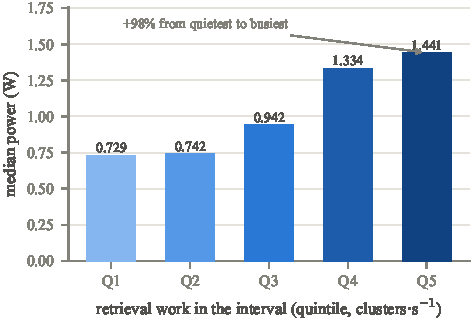
\includegraphics[width=\columnwidth]{fig7_energy.pdf}
\caption{Median power against retrieval work, measured on the unplugged
handset. The rise is what makes effort worth controlling; the quintiles are
ordered, so they take one stepped hue.}
\label{fig:energy}
\end{figure}

We report the regression behind the marginal cost as explaining $R^2 = 0.16$ of
the variance in interval power. That is low, and it is the honest figure: most
of a phone's power draw during a retrieval workload is not retrieval.

\section{A Negative Result: The Shield Reads the Wrong Thermometer}
\label{sec:sensors}

\subsection{The policy, and what it did}
\label{sec:c5}

We built a device-state policy that derates retrieval effort on thermal and
battery grounds, with a warm threshold at $42\,^{\circ}$C and a hot threshold at
$46\,^{\circ}$C. The thresholds were anchored on the one thermal measurement we
had when we wrote it: the handset's skin sensor sat at $36.6\,^{\circ}$C idle
and reached $41.4\,^{\circ}$C after 60~s of full load. $42\,^{\circ}$C is
therefore ``sustained load'', not a round number.

Run on the handset over $22.0$ minutes and $19{,}719$ decisions per arm, the
policy looks like a success on latency: it cut p95 from $84.7$ to $43.3$~ms and
deadline misses from $1.11\%$ to $0.01\%$, at a cost of $0.10$ recall. But only
$542$ of $19{,}719$ decisions---$2.7\%$---had any device signal behind them at
all. The other $97.3\%$ were taken blind and reduce to the budgeted policy. The
latency improvement is real and is not evidence for a \emph{thermal} policy.

\subsection{Why}

Figure~\ref{fig:sensors} shows the cause across every run we recorded. Android
exposes a ``skin'' temperature intended to model what a hand feels, and also
exposes per-zone sensors. On all six runs the skin sensor peaked between $34.0$
and $37.5\,^{\circ}$C while the hottest zone peaked between $54.1$ and
$78.8\,^{\circ}$C---a divergence of $20.1$ to $41.3\,^{\circ}$C.

\begin{figure}[t]
\centering
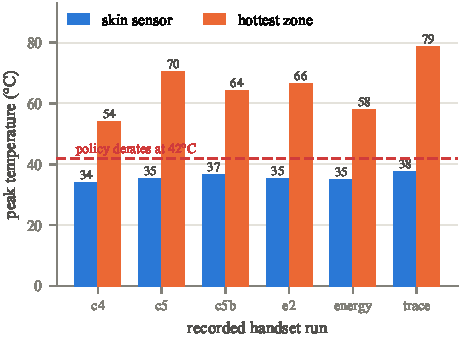
\includegraphics[width=\columnwidth]{fig5_sensors.pdf}
\caption{Peak temperature per recorded handset run, by sensor. The skin sensor
reaches the policy's $42\,^{\circ}$C derate threshold in \emph{zero} of six
runs; the hottest internal zone exceeds it in \emph{all six}. A thermal shield
calibrated on skin temperature never trips.}
\label{fig:sensors}
\end{figure}

The consequence is stark and reproducible. Figure~\ref{fig:trace} replays one
recorded run through the identical policy, changing only which sensor it reads.
Reading the skin, the threshold is never crossed and the controller spends
$97\%$ of the run at full effort. Reading the hottest zone, it derates across
$100\%$ of the run, down to the floor level, giving up $0.266$ recall against
what the latency budget alone would have allowed.

\begin{figure}[t]
\centering
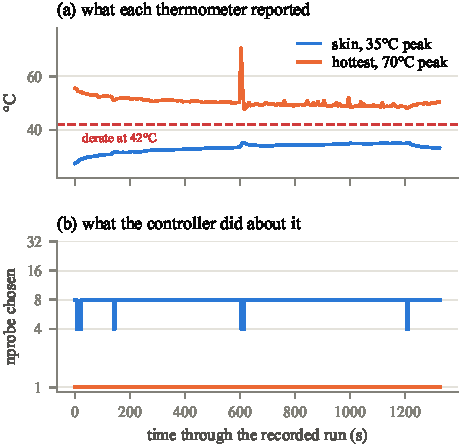
\includegraphics[width=\columnwidth]{fig8_trace.pdf}
\caption{One recorded run, one policy, two thermometers. (a) The sensors
disagree by $35.1\,^{\circ}$C at peak. (b) The resulting control decisions are
not similar: \texttt{nprobe}~$=8$ throughout on skin, \texttt{nprobe}~$=1$
throughout on the hottest zone. The choice of sensor determines the entire
behaviour of the shield.}
\label{fig:trace}
\end{figure}

\subsection{What we take from it}

Neither sensor is obviously correct. The skin sensor is the right quantity for
user comfort and is what a vendor intends a thermal policy to read; the hottest
zone is the right quantity for component stress but is a spike-prone signal
that would derate a retrieval system almost permanently under a sustained
workload. Our policy is not miscalibrated so much as pointed at a signal that
does not carry the information the shield needs at the threshold where the
shield acts.

We report this because it is the kind of result that is expensive to rediscover
and cheap to share. A practitioner building a thermally-aware mobile system
should measure both sensors on their target device before choosing thresholds,
and should expect the two to disagree by tens of degrees.

\section{Limitations}

\textbf{Generation was not run on the handset.} Retrieval, its latency and its
energy were measured on the device. \texttt{flan-t5-base} generation was run on
a host; all generation timings in this paper are host numbers and are labelled
as such. An end-to-end on-device latency figure would require a quantised
generator and is future work.

\textbf{One device, one corpus for the main result.} The profile table, the
energy measurements and the thermal runs are from a single handset model. The
allocation of Section~\ref{sec:c6} is fitted on one corpus; difficulty buckets
are a property of a particular index's cluster geometry and we refuse to load a
fit across corpora for that reason. Generality across devices and corpora is
unestablished.

\textbf{The policy comparison of Section~\ref{sec:policies} is on a different
corpus} (SIFT1M) from the profile table used elsewhere (SQuAD). The two are not
directly comparable and we do not combine them.

\textbf{Index memory footprint targets were met, but on a contended machine.}
Resident memory was $41.0$~MB against $283.0$~MB of raw vectors for one corpus
and $11.9$ against $488.3$~MB for another. The timing samples in that
acceptance run were taken with $12.4\%$ of samples above our load threshold; we
kept and labelled them rather than silently re-running.

\textbf{The thermal decomposition is refused, not merely uncertain.} We can say
what fraction of measured \emph{power} retrieval accounts for
($29.9\%$ on one trace); we cannot decompose a temperature rise, and we say so.

\textbf{The storage comparison of Section~\ref{sec:regime} is one index
configuration.} Our clusters average $216$ vectors. Per-cluster graphs may well
pay at cluster sizes large enough to amortise the cost of constructing them; our
result is that they do not at the sizes this design produces, inside the regime
where the analytic condition predicts they should.

\section{Conclusion}

A two-phase on-device vector index computes, for free, a signal that predicts
how much effort each query needs, and until now that signal was discarded. We
showed it separates recall@10 at the cheapest effort level by $3.5\times$
across difficulty quintiles, fitted an allocation against costs measured on a
physical handset, and validated on held-out queries that it beats uniform
allocation at near-equal device cost on three of five budgets.

We also showed a thermal shield failing for a reason worth publishing: the
sensor a mobile platform makes conventional never reaches the threshold at
which the shield is calibrated to act, while an internal zone on the same
device exceeds it on every recorded run. We report that failure with the same
apparatus we used for the successes, which is the point of building the
apparatus.

\section*{Artifact Availability}

All experiments are reproducible from the released repository. Each figure and
table in this paper is generated by a script that reads a JSON or Parquet file
written by a recorded run; the expensive measurement underlying
Section~\ref{sec:c6} is cached so the allocation and its verdict can be
re-derived in seconds from identical numbers. The test suite comprises $599$
tests, and an end-to-end verification harness re-runs every acceptance gate.

% If the last references still spill onto a page of their own, uncomment ONE of
% these before recompiling. Both are typographic, not content changes.
%   \footnotesize        % sets the whole bibliography one size smaller
%   \IEEEtriggeratref{13}  % forces the column break at [13] to balance the list
\begin{thebibliography}{00}

\bibitem{lewis2020rag}
P.~Lewis \emph{et al.}, ``Retrieval-augmented generation for knowledge-intensive
NLP tasks,'' in \emph{Advances in Neural Information Processing Systems},
vol.~33, 2020, pp.~9459--9474.

\bibitem{park2025mobilerag}
J.~Park, S.~Lee, and H.~Kim, ``MobileRAG: Enabling efficient
retrieval-augmented generation on mobile devices,'' arXiv:2507.01079, 2025.

\bibitem{malkov2020hnsw}
Y.~A. Malkov and D.~A. Yashunin, ``Efficient and robust approximate nearest
neighbor search using hierarchical navigable small world graphs,'' \emph{IEEE
Trans. Pattern Anal. Mach. Intell.}, vol.~42, no.~4, pp.~824--836, 2020.

\bibitem{johnson2021faiss}
J.~Johnson, M.~Douze, and H.~J\'egou, ``Billion-scale similarity search with
GPUs,'' \emph{IEEE Trans. Big Data}, vol.~7, no.~3, pp.~535--547, 2021.

\bibitem{douze2024faiss}
M.~Douze \emph{et al.}, ``The Faiss library,'' arXiv:2401.08281, 2024.

\bibitem{subramanya2019diskann}
S.~Jayaram Subramanya, F.~Devvrit, H.~V. Simhadri, R.~Krishnaswamy, and
R.~Kadekodi, ``DiskANN: Fast accurate billion-point nearest neighbor search on
a single node,'' in \emph{Advances in Neural Information Processing Systems},
vol.~32, 2019.

\bibitem{li2020earlytermination}
C.~Li, M.~Zhang, D.~G. Andersen, and Y.~He, ``Improving approximate nearest
neighbor search through learned adaptive early termination,'' in \emph{Proc.
ACM SIGMOD Int. Conf. Management of Data}, 2020, pp.~2539--2554.

\bibitem{guo2020scann}
R.~Guo, P.~Sun, E.~Lindgren, Q.~Geng, D.~Simcha, F.~Chern, and S.~Kumar,
``Accelerating large-scale inference with anisotropic vector quantization,'' in
\emph{Proc. Int. Conf. Machine Learning}, 2020, pp.~3887--3896.

\bibitem{rajpurkar2016squad}
P.~Rajpurkar, J.~Zhang, K.~Lopyrev, and P.~Liang, ``SQuAD: 100,000+ questions
for machine comprehension of text,'' in \emph{Proc. Conf. Empirical Methods in
Natural Language Processing}, 2016, pp.~2383--2392.

\bibitem{chung2024flan}
H.~W. Chung \emph{et al.}, ``Scaling instruction-finetuned language models,''
\emph{J. Mach. Learn. Res.}, vol.~25, no.~70, pp.~1--53, 2024.

\bibitem{jeong2024adaptiverag}
S.~Jeong, J.~Baek, S.~Cho, S.~J. Hwang, and J.~C. Park, ``Adaptive-RAG:
Learning to adapt retrieval-augmented large language models through question
complexity,'' in \emph{Proc. NAACL-HLT}, 2024, pp.~7036--7050.

\bibitem{asai2024selfrag}
A.~Asai, Z.~Wu, Y.~Wang, A.~Sil, and H.~Hajishirzi, ``Self-RAG: Learning to
retrieve, generate, and critique through self-reflection,'' in \emph{Proc.
Int. Conf. Learning Representations}, 2024.

\bibitem{jiang2023flare}
Z.~Jiang, F.~F. Xu, L.~Gao, Z.~Sun, Q.~Liu, J.~Dwivedi-Yu, Y.~Yang, J.~Callan,
and G.~Neubig, ``Active retrieval augmented generation,'' in \emph{Proc. Conf.
Empirical Methods in Natural Language Processing}, 2023, pp.~7969--7992.

\bibitem{mallen2023whennot}
A.~Mallen, A.~Asai, V.~Zhong, R.~Das, D.~Khashabi, and H.~Hajishirzi, ``When
not to trust language models: Investigating effectiveness of parametric and
non-parametric memories,'' in \emph{Proc. Annu. Meeting Assoc. Computational
Linguistics}, 2023, pp.~9802--9822.

\bibitem{seemakhupt2024edgerag}
K.~Seemakhupt, S.~Liu, and S.~Khan, ``EdgeRAG: Online-indexed RAG for edge
devices,'' arXiv:2412.21023, 2024.

\bibitem{chatzakis2025darth}
M.~Chatzakis, Y.~Papakonstantinou, and T.~Palpanas, ``DARTH: Declarative recall
through early termination for approximate nearest neighbor search,''
\emph{Proc. ACM Manag. Data}, vol.~3, no.~4, Art.~242, 2025.

\bibitem{chen2021spann}
Q.~Chen, B.~Zhao, H.~Wang, M.~Li, C.~Liu, Z.~Li, M.~Yang, and J.~Wang, ``SPANN:
Highly-efficient billion-scale approximate nearest neighbor search,'' in
\emph{Advances in Neural Information Processing Systems}, vol.~34, 2021.

\bibitem{aumuller2020annbench}
M.~Aum\"uller, E.~Bernhardsson, and A.~Faithfull, ``ANN-Benchmarks: A
benchmarking tool for approximate nearest neighbor algorithms,'' \emph{Inf.
Syst.}, vol.~87, Art.~101374, 2020.

\bibitem{karpukhin2020dpr}
V.~Karpukhin, B.~O\u{g}uz, S.~Min, P.~Lewis, L.~Wu, S.~Edunov, D.~Chen, and
W.~Yih, ``Dense passage retrieval for open-domain question answering,'' in
\emph{Proc. Conf. Empirical Methods in Natural Language Processing}, 2020,
pp.~6769--6781.

\bibitem{li2023gte}
Z.~Li, X.~Zhang, Y.~Zhang, D.~Long, P.~Xie, and M.~Zhang, ``Towards general
text embeddings with multi-stage contrastive learning,'' arXiv:2308.03281,
2023.

\bibitem{gao2023ragsurvey}
Y.~Gao \emph{et al.}, ``Retrieval-augmented generation for large language
models: A survey,'' arXiv:2312.10997, 2023.

\bibitem{laskaridis2024melt}
S.~Laskaridis, K.~Katevas, L.~Minto, and H.~Haddadi, ``MELTing point: Mobile
evaluation of language transformers,'' in \emph{Proc. ACM Int. Conf. Mobile
Computing and Networking}, 2024.

\bibitem{ignatov2019aibench}
A.~Ignatov \emph{et al.}, ``AI benchmark: All about deep learning on smartphones
in 2019,'' in \emph{Proc. IEEE/CVF Int. Conf. Computer Vision Workshops},
2019, pp.~3617--3635.

\bibitem{strubell2019energy}
E.~Strubell, A.~Ganesh, and A.~McCallum, ``Energy and policy considerations for
deep learning in NLP,'' in \emph{Proc. Annu. Meeting Assoc. Computational
Linguistics}, 2019, pp.~3645--3650.

\bibitem{schwartz2020greenai}
R.~Schwartz, J.~Dodge, N.~A. Smith, and O.~Etzioni, ``Green AI,''
\emph{Commun. ACM}, vol.~63, no.~12, pp.~54--63, 2020.

\end{thebibliography}

\balance
\end{document}
